% The four cases of core specialization (docs/source/schedule_optimization_formulation.md, section 3.1).
% Build: pdflatex core_specialization_cases.tex && pdftocairo -svg core_specialization_cases.pdf
\documentclass[tikz,border=6pt]{standalone}
\usepackage{amsmath,amssymb}
\usetikzlibrary{arrows.meta,calc}

\definecolor{opA}{RGB}{52,112,180}
\definecolor{opAb}{RGB}{150,190,230}
\definecolor{opB}{RGB}{60,150,90}
\definecolor{opC}{RGB}{220,130,40}
\definecolor{corefill}{RGB}{245,245,248}
\definecolor{memfill}{RGB}{255,250,230}
\definecolor{ok}{RGB}{40,130,60}
\definecolor{warn}{RGB}{190,50,40}
\definecolor{muted}{RGB}{110,110,110}

\tikzset{
  tile/.style={draw=black!60, line width=0.3pt, minimum size=0pt},
  core/.style={draw=black!70, rounded corners=3pt, fill=corefill, line width=0.6pt},
  mem/.style={draw=black!50, rounded corners=2pt, fill=memfill, line width=0.4pt},
  chip/.style={draw=black!50, fill=white, rounded corners=1pt, inner sep=1.5pt, font=\scriptsize},
  other/.style={draw=black!40, rounded corners=3pt, fill=black!5, font=\scriptsize, text=muted, align=center},
  flow/.style={-{Stealth[length=2.2mm]}, line width=0.6pt, black!70},
  link/.style={-{Stealth[length=2.2mm]}, line width=0.9pt, black!70},
  dep/.style={-{Stealth[length=1.4mm]}, line width=0.35pt, black!45},
  title/.style={font=\bfseries\small, anchor=west},
  target/.style={font=\scriptsize, anchor=west, align=left},
  badge/.style={font=\scriptsize\bfseries, rounded corners=2pt, inner sep=2pt, text=white},
}

% \tile{x}{y}{color}: one tile, 0.34 x 0.34.
\newcommand{\tile}[3]{\fill[#3] (#1,#2) rectangle ++(0.34,0.34); \draw[tile] (#1,#2) rectangle ++(0.34,0.34);}
% \slice{x}{color}: one task on a core's timeline.
\newcommand{\slice}[2]{\fill[#2] (#1,2.95) rectangle ++(0.33,0.32); \draw[tile] (#1,2.95) rectangle ++(0.33,0.32);}
% Common panel frame: core box, timeline axis, memory box.
\newcommand{\coreframe}[1]{%
  \draw[core] (2.3,1.25) rectangle (5.15,3.95);
  \node[font=\scriptsize, anchor=north west] at (2.35,3.93) {#1};
  \draw[-{Stealth[length=1.2mm]}, black!40, line width=0.3pt] (2.45,2.85) -- (5.0,2.85);
  \node[font=\tiny, text=muted, anchor=north east] at (5.02,2.84) {time};
  \draw[mem] (2.45,1.38) rectangle (5.0,2.42);
  \node[font=\tiny, text=muted, anchor=north west] at (2.47,2.41) {local memory};
}

\begin{document}
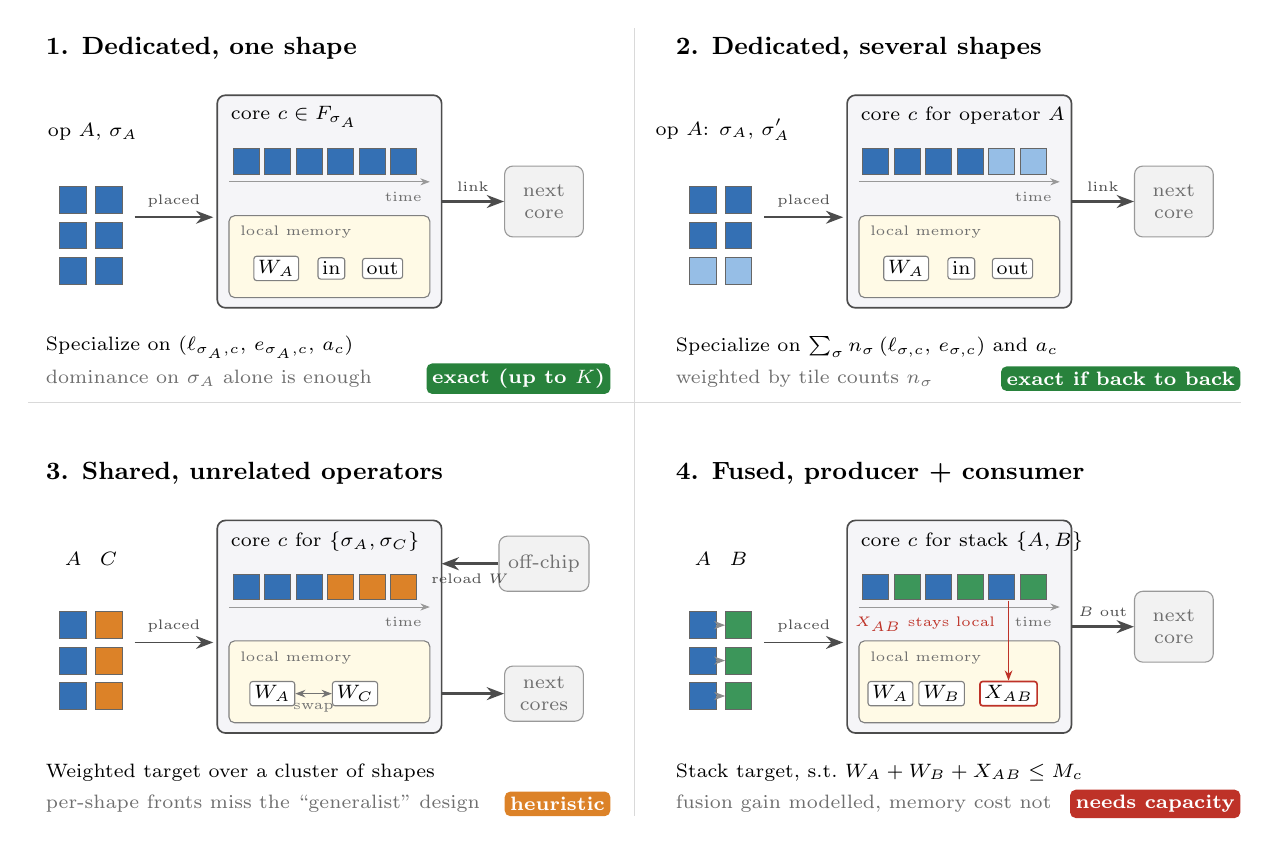
\begin{tikzpicture}[x=1cm,y=1cm]

% ------------------------------------------------------------------ case 1 ----
\begin{scope}[shift={(0,0)}]
  \node[title] at (0,4.55) {1. Dedicated, one shape};
  \node[font=\scriptsize, anchor=south] at (0.72,3.25) {op $A$, $\sigma_A$};
  \foreach \i in {0,1,2} { \tile{0.3}{1.55+0.45*\i}{opA} \tile{0.75}{1.55+0.45*\i}{opA} }
  \draw[flow] (1.25,2.4) -- node[above, font=\tiny] {placed} (2.25,2.4);
  \coreframe{core $c \in F_{\sigma_A}$}
  \foreach \i in {0,...,5} { \slice{2.5+0.4*\i}{opA} }
  \node[chip] at (3.05,1.75) {$W_A$};
  \node[chip] at (3.75,1.75) {in};
  \node[chip] at (4.4,1.75) {out};
  \node[other, minimum width=1.0cm, minimum height=0.9cm] (n1) at (6.45,2.6) {next\\core};
  \draw[link] (5.15,2.6) -- node[above, font=\tiny] {link} (n1.west);
  \node[target] at (0,0.75) {Specialize on $(\ell_{\sigma_A,c},\, e_{\sigma_A,c},\, a_c)$};
  \node[target, text=muted] at (0,0.35) {dominance on $\sigma_A$ alone is enough};
  \node[badge, fill=ok, anchor=east] at (7.3,0.35) {exact (up to $K$)};
\end{scope}

% ------------------------------------------------------------------ case 2 ----
\begin{scope}[shift={(8.0,0)}]
  \node[title] at (0,4.55) {2. Dedicated, several shapes};
  \node[font=\scriptsize, anchor=south] at (0.72,3.25) {op $A$: $\sigma_A$, $\sigma_A'$};
  \foreach \i in {1,2} { \tile{0.3}{1.55+0.45*\i}{opA} \tile{0.75}{1.55+0.45*\i}{opA} }
  \tile{0.3}{1.55}{opAb} \tile{0.75}{1.55}{opAb}
  \draw[flow] (1.25,2.4) -- node[above, font=\tiny] {placed} (2.25,2.4);
  \coreframe{core $c$ for operator $A$}
  \foreach \i in {0,...,3} { \slice{2.5+0.4*\i}{opA} }
  \slice{4.1}{opAb} \slice{4.5}{opAb}
  \node[chip] at (3.05,1.75) {$W_A$};
  \node[chip] at (3.75,1.75) {in};
  \node[chip] at (4.4,1.75) {out};
  \node[other, minimum width=1.0cm, minimum height=0.9cm] (n2) at (6.45,2.6) {next\\core};
  \draw[link] (5.15,2.6) -- node[above, font=\tiny] {link} (n2.west);
  \node[target] at (0,0.75) {Specialize on $\sum_\sigma n_\sigma\,(\ell_{\sigma,c},\, e_{\sigma,c})$ and $a_c$};
  \node[target, text=muted] at (0,0.35) {weighted by tile counts $n_\sigma$};
  \node[badge, fill=ok, anchor=east] at (7.3,0.35) {exact if back to back};
\end{scope}

% ------------------------------------------------------------------ case 3 ----
\begin{scope}[shift={(0,-5.4)}]
  \node[title] at (0,4.55) {3. Shared, unrelated operators};
  \node[font=\scriptsize, anchor=south] at (0.47,3.25) {$A$};
  \node[font=\scriptsize, anchor=south] at (0.92,3.25) {$C$};
  \foreach \i in {0,1,2} { \tile{0.3}{1.55+0.45*\i}{opA} \tile{0.75}{1.55+0.45*\i}{opC} }
  \draw[flow] (1.25,2.4) -- node[above, font=\tiny] {placed} (2.25,2.4);
  \coreframe{core $c$ for $\{\sigma_A, \sigma_C\}$}
  \slice{2.5}{opA} \slice{2.9}{opA} \slice{3.3}{opA}
  \slice{3.7}{opC} \slice{4.1}{opC} \slice{4.5}{opC}
  \node[chip] (wa3) at (3.0,1.75) {$W_A$};
  \node[chip] (wc3) at (4.05,1.75) {$W_C$};
  \draw[{Stealth[length=1.3mm]}-{Stealth[length=1.3mm]}, black!55, line width=0.4pt] (wa3.east) -- node[below, font=\tiny] {swap} (wc3.west);
  \node[other, minimum width=1.0cm, minimum height=0.7cm] (off3) at (6.45,3.4) {off-chip};
  \node[other, minimum width=1.0cm, minimum height=0.7cm] (n3) at (6.45,1.75) {next\\cores};
  \draw[link] (off3.west) -- node[below, font=\tiny] {reload $W$} (5.15,3.4);
  \draw[link] (5.15,1.75) -- (n3.west);
  \node[target] at (0,0.75) {Weighted target over a cluster of shapes};
  \node[target, text=muted] at (0,0.35) {per-shape fronts miss the ``generalist'' design};
  \node[badge, fill=opC, anchor=east] at (7.3,0.35) {heuristic};
\end{scope}

% ------------------------------------------------------------------ case 4 ----
\begin{scope}[shift={(8.0,-5.4)}]
  \node[title] at (0,4.55) {4. Fused, producer + consumer};
  \node[font=\scriptsize, anchor=south] at (0.47,3.25) {$A$};
  \node[font=\scriptsize, anchor=south] at (0.92,3.25) {$B$};
  \foreach \i in {0,1,2} {
    \tile{0.3}{1.55+0.45*\i}{opA} \tile{0.75}{1.55+0.45*\i}{opB}
    \draw[dep] (0.64,1.72+0.45*\i) -- (0.75,1.72+0.45*\i);
  }
  \draw[flow] (1.25,2.4) -- node[above, font=\tiny] {placed} (2.25,2.4);
  \coreframe{core $c$ for stack $\{A, B\}$}
  \foreach \i in {0,1,2} { \slice{2.5+0.8*\i}{opA} \slice{2.9+0.8*\i}{opB} }
  \node[chip] (wa4) at (2.85,1.75) {$W_A$};
  \node[chip] (wb4) at (3.5,1.75) {$W_B$};
  \node[chip, draw=warn, line width=0.6pt] (x4) at (4.35,1.75) {$X_{AB}$};
  \draw[-{Stealth[length=1.3mm]}, warn, line width=0.5pt] (4.35,2.93) -- (x4.north);
  \node[font=\tiny, text=warn, anchor=east] at (4.3,2.63) {$X_{AB}$ stays local};
  \node[other, minimum width=1.0cm, minimum height=0.9cm] (n4) at (6.45,2.6) {next\\core};
  \draw[link] (5.15,2.6) -- node[above, font=\tiny] {$B$ out} (n4.west);
  \node[target] at (0,0.75) {Stack target, s.t.\ $W_A + W_B + X_{AB} \le M_c$};
  \node[target, text=muted] at (0,0.35) {fusion gain modelled, memory cost not};
  \node[badge, fill=warn, anchor=east] at (7.3,0.35) {needs capacity};
\end{scope}

% Separators.
\draw[black!15, line width=0.4pt] (7.6,-5.2) -- (7.6,4.8);
\draw[black!15, line width=0.4pt] (-0.1,0.05) -- (15.3,0.05);

\end{tikzpicture}
\end{document}
